\begin{center}
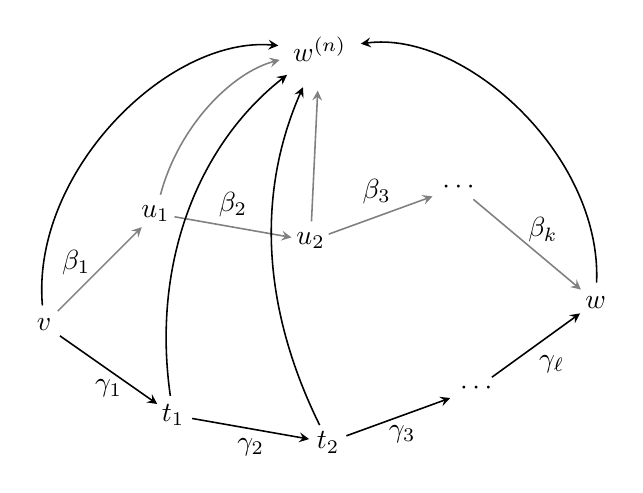
\begin{tikzpicture}[line width = 0.2mm, >=stealth, shorten >= 7pt, shorten <=7pt]
\draw[->, Black!50!White] (0,0) coordinate (a1)
-- node[above, xshift = -0.3cm, yshift = -0.2cm] {$\textcolor{Black}{\beta_1}$} ++(45:2) coordinate (a2);
\draw[->, Black!50!White,] (a2)
-- node[above] {$\textcolor{Black}{\beta_2}$} ++(-10:2) coordinate (a3);
\draw[->, Black!50!White, shorten >= 10pt] (a3)
-- node[above, xshift = -0.1cm] {$\textcolor{Black}{\beta_3}$} ++(20:2) coordinate (a4);
\draw[->, Black!50!White] (a4)
-- node[above, xshift = 0.2cm, yshift = -0.1cm] {$\textcolor{Black}{\beta_k}$}++(-40:2.275) coordinate (a5);
\node at (a1) {$v$};
\node at (a2) {$u_1$};
\node at (a3) {$u_2$};
\node at (a4) {$\cdots$};
\node at (a5) {$w$};

\draw[->] (0,0)
-- node[below] {$\gamma_1$}++(-35:2) coordinate (a6);
\draw[->] (a6)
-- node[below] {$\gamma_2$}++(-10:2) coordinate (a7);
\draw[->, shorten >= 10pt] (a7)
-- node[below] {$\gamma_3$}++(20:2) coordinate (a8);
\draw[->] (a8)
-- node[below, xshift = 0.2cm] {$\gamma_{\ell}$} (a5);
\node at (a6) {$t_1$};
\node at (a7) {$t_2$};
\node at (a8) {$\cdots$};
\coordinate (a9) at (3.5,3.5);
\node at (a9) {$w^{(n)}$};
\foreach \n/\ang/\col in {1/50/{Black},2/30/{Black!50!White}, 3/0/{Black!50!White}, 5/-50/{Black}, 6/30/{Black}, 7/25/{Black}}{
\draw[->, \col, shorten >= 15pt] (a\n) to[bend left = \ang] (a9);
}
\end{tikzpicture}
\end{center}